\section{About Box}{
		\begin{figure}
		\centering
		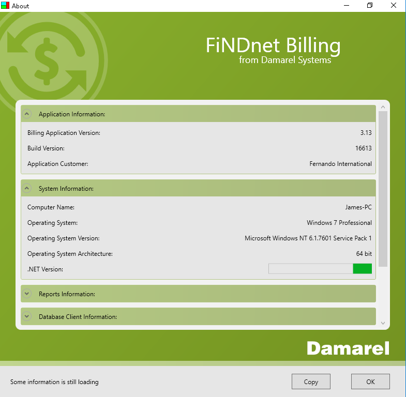
\includegraphics[width=0.75\textwidth]{AboutBox}
		\caption{A Screenshot of the About box window}
		\label{fig:AboutBox}
	\end{figure}
	Next I had to create a new WPF about box to replace the old about box written in Centura. The aims of this project was to be able to provide more debugging information about the environment set up to our customers and support team. This was developed using MVVM. Meaning I had to learn a lot of WPF mainly about how the XAML works and the different features which were available in it for example I had to use triggers to change the display format depending on the value of a property in the view model. This project was completed and included in the Billing release.
}
